\documentclass[a4paper,11pt,twoside]{report}
\usepackage[left=2.5cm,right=2cm,top=2cm,bottom=2cm]{geometry}
\usepackage{ntheorem}
\usepackage{amsmath}
\usepackage{amssymb}
\usepackage{indentfirst}
\usepackage{stmaryrd}
\usepackage{verbatimbox}
\usepackage{amsfonts}
\usepackage{proof}
\usepackage{graphicx}
\usepackage{subfig}
\usepackage{mathtools}
\usepackage{comment}
\usepackage{qtree}

\newtheorem{def1}{\textbf{Definition}}[chapter]
\newtheorem{exmp}{\textit{Example}}[section]


\begin{document}

\pagenumbering{roman}
\tableofcontents

\relax

\chapter*{Abstract}
\addcontentsline{toc}{chapter}{\numberline{}Abstract}

\chapter*{Acknowledgements}
\addcontentsline{toc}{chapter}{\numberline{}Acknowledgements}
\chapter*{Introduction}
\addcontentsline{toc}{chapter}{\numberline{}Introduction}


\chapter{Lambda Calculus}

\pagenumbering{arabic}
The Lambda Calculus is an example of a formal system which consists a language of lambda terms and some auxiliary notions such as \textit{free variables} and \textit{subterms}, and the transformation theory. The core of the theory is the notion of substitution - the driving force behind function application. 


\section{$\lambda$-terms}

\noindent The expressions in lambda calculus can be formalized into following: 


\begin{def1}
\normalfont \textbf{($\lambda$-TERMS)} $\lambda$-terms can be defined by the following rules:
\end{def1}

\begin{itemize}
\item a variable, $x$, itself is a lambda term
\item if $M$ is a lambda term, and $x$ is a variable, then $(\lambda x.M)$ is a lambda term
\item if $M$ and $N$ are both lambda terms, then \textit{(MN)} is a lambda term
\end{itemize}
A lambda term is valid if and only if it can be obtained by repeated application of these rules. However, some parentheses can be omitted in certain forms. For example the leftmost, outermost brackets are usually omitted.

\textbf{A lambda abstraction $\lambda x.M$} takes a single input x and returns a term M. Thus, it defines an \textbf{anonymous} function. For example $\lambda x.x^2$ is a lambda abstraction for the function $f(x) = x^2$ using the term $x^2$ for M, then we can say that $f = \lambda x.x^2$. The function is anonymous since we write $(x^2)2$ rather than $f3$.

\textbf{An application $(MN)$} applies the input term N to the function M. For example $(\lambda x.x^2)2$ is an application that applies 2 to the function $f(x) = x^2$, it return $2^2$ which equals 4.

As mentioned above, leftmost, outermost brackets are usually omitted. Therefore, $M_1M_2(M_3M_4)$ stands for $((M_1\cdot M_2)(M_3\cdot M_4))$. Similarly, $\lambda$ can be omitted in repeated abstractions, for example $\lambda x_1x_2.M$ stands for $\lambda x_1.(\lambda x_2.M)$.

\begin{def1}
\normalfont \textbf{(free and bound variables)} The set of free and bound variables are defined inductively by the following function:
\end{def1}

\begin{equation*}\label{eq:fv}
\begin{array}{lcllcl}
FV(x)           & = & \{x\}             & BV(x)           &=& \emptyset\\
FV(\lambda x.M) & = & FV(M)\backslash \{x\} & BV(\lambda x.M) &=& BV(M)\cup \{x\}\\
FV(MN)          & = & FV(M)\cup FV(N) & BV(MN)          &=& BV(M)\cup BV(N)
\end{array}
\end{equation*}


For example, the lambda term $\lambda x.x$ has no free variables but a bound variable $x$. The function $\lambda x.x+y$ only has a single free variable $y$ and a bound variable $x$. 
Notice that, the sets of bound and free variables are not necessarily disjoint; $x$ occurs both bound and free in:
\begin{equation*}
x(\lambda xy.x)
\end{equation*}


\section{Substitution}

\noindent A cursory approach to define the substitution operation leads to the problem of \textit{variable capture}. It occurs when we substitute a term containing a free variable into a scope where the variable becomes bound. For example:
\begin{equation*}
(\lambda xy.xy)y \neq \lambda y.yy
\end{equation*} 

The free occurrence of y in the left hand term becomes confused with the bound variable after substitution.To avoid \textit{variable capture}, we define a capture-avoiding substitution. The notion $[x:=N]$ indicates the replacement of a variable $x$ by a term $N$:

\begin{equation*}
\begin{array}{lrll}
(1)&x[x:=N]&=N & ~\\
(2)&y[x:=N]&=y,& if\ y\neq x\\
(3)&(\lambda y.M)[x:=N]&=\lambda y.M,& if\ y=x\\
(4)&(\lambda y.M)[x:=N]&=\lambda y.(M[x:=N]),& if\ y\notin FV(N)\ \& \ y\neq x\\
(5)&(\lambda y.M)[x:=N]&=\lambda z.(M[y:=z])[x:=N],& if\ y\in FV(N)\ \& \ y\neq x,z\  new\\
(6)&(M_1M_2)[x:=N] &= (M_1[x:=N])(M_2[x:=N])&
\end{array}
\end{equation*}

\begin{def1}\label{def1}
\normalfont \textbf{($\alpha$-equivalent)} \textit{$M$ is $\alpha$-equivalent to $N$, written $M$ $\equiv_\alpha N$, if $N$ results from $M$ by a series of changes of bound variable.}
\end{def1}

The notion of alpha-equivalent(or congruence) is a basic form of equivalence defined in lambda calculus. It captures the property that the particular choice of a bound variable in a lambda abstraction does not matter. For instance, $\lambda x.x$ and $\lambda y.y$ are $\alpha$-congruent lambda terms which represent the same function. Notice that, the term-variable $x$ and $y$ are not $\alpha$-equivalent terms since they are not bound in a lambda abstraction.

With the property of alpha equivalence, we can define the \textit{$\alpha$-conversion}:

\begin{equation*}
\lambda x.M =_\alpha \lambda z.(M[z:=x])
\end{equation*}

In some sense, the $\alpha$-conversion is defined by the spirit of the (5) substitution rule. If we have a function $\lambda x.M$, then we can apply a substitution to this function: $(\lambda x.M)[z:=x]$. According to the fifth substitution rule, it is unfolded to $(\lambda z.M[z:=x])$. Using the $\alpha$-conversion, we can always rename the bound variables of a term. 

\begin{def1}
\normalfont \textbf{(Variable Convention\cite{hankin1994lambda})} \textit{If $M_1$,...,$M_n$ occur in a certain context then in these terms all bound variables are chosen to be different from free variables.}
\end{def1}

The alpha-conversion is built based on the variable convention. Alpha convertion is used to allow bound variable names to be changed. For example, alpha-conversion of $\lambda x.x$ might get $\lambda y.y$. Terms that differ only by alpha-conversion are called alpha-equivalence(or alpha-congruence) as mentioned in the definition \ref{def1}. By the assumption that free and bound variables are always different(variable convention), and that alpha-conversion will take place whenever a variable is both free and bound. The definition of term substitution becomes:
\begin{equation*}
\begin{array}{rll}
x[x:=N]&=N & ~\\
y[x:=N]&=y,& if\ y\neq x\\
(\lambda y.M)[x:=N]&=\lambda y.(M[x:=N])& \\
(M_1M_2)[x:=N] &= (M_1[x:=N])(M_2[x:=N])&
\end{array} 
\end{equation*}

By this definition of term substitution, the \textit{variable capture} is avoided. Since that y is bound in $\lambda y.M$ of the context:
\begin{equation*}
\lambda y.M[x:=N]
\end{equation*}
y can only be bound in N according to variable convention rule, otherwise, if y is also free in N, it would be renamed by another variable. 

Here is an example of its use:
\begin{equation*}
\begin{array}{ll}
&(\lambda xyz.xzy)(\lambda xz.x)\\
=& \lambda yz.(\lambda xz.x)zy \\
=& \lambda yz.(\lambda xw.x)zy\ \ by\ the\ variable\ convention \\
=& \lambda yz.(\lambda w.z)y\\
=& \lambda yz.z\\
\end{array}
\end{equation*}

\section{$\beta$-reduction}

\noindent There are various notions of reduction for $\lambda$-terms, but the principle one is $\beta$-reduction. $\beta$-reduction is the one-step reduction relation, written as $'\rightarrow _\beta'$. 

\begin{def1}
($\beta$-reduction) For $\lambda$-terms $M$ and $N$, we say that $M$ $\beta$-reduces in one step to $N$, written as $M \rightarrow _\beta N$:
\end{def1}
\begin{equation*}
(\lambda x.M)N\rightarrow _\beta M[x:=N]
\end{equation*}

\begin{equation*}
\frac{M\rightarrow _\beta N}{MZ \rightarrow _\beta NZ}
\end{equation*}
\begin{equation*}
\frac{M\rightarrow _\beta N}{ZM \rightarrow _\beta ZM}
\end{equation*}
\begin{equation*}
\frac{M\rightarrow _\beta N}{\lambda x.M \rightarrow _\beta \lambda x.N}
\end{equation*}

\noindent The reduction relation, written $'\twoheadrightarrow _\beta'$, is the reflexive, transitive closure of the one-step reduction relation. The one-step reduction relation allows a single step of reduction, while the reduction relation allows many steps. The reflexive transitive closure is defined as follows:
\begin{equation*}
\frac{M\rightarrow _\beta N}{M \twoheadrightarrow _\beta N}
\end{equation*}
\begin{equation*}
M \twoheadrightarrow _\beta M
\end{equation*}
\begin{equation*}
\frac{M\twoheadrightarrow _\beta N\ \ \ \ N\twoheadrightarrow _\beta Z}{M \twoheadrightarrow _\beta Z}
\end{equation*}

For the notion $'M\rightarrow _\beta N'$, it is read as '$M$ $\beta$-reduces to $N$'. The first rule defines that the reduction relation is reflexive to one-step reduction relation, while the third rule indicates the transitivity of reduction relation.

\noindent Finally, the $\beta$-equality, written as '$=_\beta$'. For $\lambda$-terms $A$ and $B$, we say that $A =_\beta B$ if either $A \equiv B$ or there exists a sequence of reduction starting with $A$, ending with $B$. It is the equivalence relation generated by $\twoheadrightarrow _\beta$:

\begin{equation*}
\frac{M\twoheadrightarrow _\beta N}{M = _\beta N}
\end{equation*}
\begin{equation*}
\frac{M = _\beta N}{N = _\beta M}
\end{equation*}
\begin{equation*}
\frac{M = _\beta N\ \ \ \ N = _\beta Z}{M = _\beta Z}
\end{equation*}

For the notion $'M = _\beta N'$, we say '$M$ $\beta$-equivalent to $N$'. 

\noindent Following is a simple example which applies $\beta$-reduction:

\begin{equation*}
\begin{array}{ll}
&(\lambda x.x^2)3\\
=& (x^2)[x:=3] \\
=& 3^2 \\
=&9 \\
\end{array}
\end{equation*}


\begin{def1}
($\beta$-redex) A $\beta$-redex of a $\lambda$-term $M$ is a subterm of M of the form ($\lambda$x.P)Q. A term M is called in $\beta$-normal form if it has no $\beta$-redex.
\end{def1}
A $\beta$-redex is essentially a candidate for an application of $\beta$-reduction. A term $M$ has a $\beta$-normal form if there exists a term N such that N is in $\beta$-normal form and $M \twoheadrightarrow _\beta N$. 

\section{Head Normal Form}

\noindent A $\lambda$-term in head normal form is generally in the form:

\begin{equation*}
\lambda x_1\ldots x_n.xM_1\ldots M_m\ \ \ \ \ \ \ \ n,m\geqslant 0
\end{equation*}

In this case $x$ is called the head variable. If $M \equiv \lambda x_1\ldots x_n.(\lambda x.M_0)M_1\ldots M_m$ where $n\geqslant 0$, $m\geqslant 1$ then the subterm $(\lambda x.M_0)M_1$ is called the head redex of $M$. Following are some examples of $\lambda$-terms in head normal form:
\begin{equation*}
(1)\ xM\ \ \ \ (2)\ \lambda x.x\ \ \ \ (3)\ \lambda xy.x((\lambda z.z)y)
\end{equation*}Normal order:
Notice that, an expression in head normal form may contain redexes in argument positions whereas a normal form may not.


\section{Reduction strategies}\label{sec:reductionstrategy}
\noindent Recall that a term is said to be in $\beta$-normal form if it has no $\beta$-redexes, that is, subterms of the shape ($\lambda$x.M)N. A term has a $\beta$-normal form if it can be reduced to a term in $\beta$ in $\beta$-normal form. It is clear that if a term has a $\beta$-normal form, then we can get to the $\beta$-normal form by exhaustively reducing all $\beta$-redexes of the term, then reducing all $\beta$-redexes of all resulting terms, and so forth until we get the $\beta$-normal form. A \textbf{$\beta$-reduction strategy} is a function that selects, whenever a term has multiple $\beta$-redexes, which one should be reduced first. If a term is in $\beta$-normal form, then no $\beta$-reduction is to be done. Notice that, a $\beta$-reduction strategy may or may not have the property that adhering to the strategy will ensure that we(eventually) reach a $\beta$-normal form, if one exists. 

In general, there are several different $\beta$-reductions possible for a given term. In this project, there are 5 different reduction strategies studied and implemented: normal order, call-by-name, call-by-value, head reduction, and applicative order. Figure X generally summarizes and compares the property of different strategies:
 
\begin{center}
\begin{table}[ht!]
\begin{tabular}{|c|c|c|c|}\hline
Reduction Strategy & Reduction Order & Reach $\beta$-normal form & Form Reached\\ \hline
Normal Order & leftmost outermost & Yes & normal form\\ \hline
Call-by-name & leftmost outermost & No  & weak head normal form\\ \hline
Call-by-value & leftmost innermost & No & weak normal form\\ \hline
Head Reduction & inside lambda abstractions & No & head normal form\\ \hline
Applicative Order & leftmost innermost & Yes & normal form\\ \hline
\end{tabular}
\caption{Reduction Strategies}
\end{table}
\end{center}

Lambda terms are modeled as Haskell constructed data, representing variable names by character:

\begin{verbatim}
type Name = Char  

data Term = Var Name | Abs Name Term | App Term Term
            deriving (Show, Eq)
\end{verbatim}


\subsection*{Operational Semantics}

A sequence of computational steps of a valid program is the operational semantics for the programming language. The final step of a terminating sequence returns the resulting value of the program. Operational semantics can be classified into two types: \textbf{structural operational semantics(SOS or small-step semantics)} and \textbf{natural semantics(NS or big-step semantics)}. The structural operational semantics describes each single step of a computation in a program, while the natural semantics describes the overall resulting value generated by the program. Following, we use both SOS and NS to define the behaviour of each reduction strategy. The small-step semantics gives reduction rules of the strategy, when the big-step semantics describes how the final term is reached.  

\subsection*{Recursion}

Although a reduction strategy may or may not have the property that ensures it reaches a $\beta$-normal form, it would recursively contract the selected redex until no redex(decided by specific reduction strategy) can be contracted. All the following Haskell functions defined corresponding to the reduction strategy model the small-step semantics. Therefore, in order to recursively reduce a $\lambda$-term, an auxiliary function \verb|recur_eval :: Term -> IO()| is defined:

\begin{verbatim}
       recur_eval :: Term -> IO()
       recur_eval t | evalcbn t == t = putStrLn("")
                    | otherwise = do
                                putStrLn("==> "++ tostring (evalcbn t))
                                recur_eval (evalcbn t)
\end{verbatim}

The Haskell function above defines the recursive reduction using Call-by-Name strategy. It uses the small-step function defined in Section \ref{subsec:cbn}. The recursion will terminate if the input $\lambda$-term cannot be reduced further, otherwise, it would print-out the term after a single step reduction and continue reducing the resulting term.



\subsection{Normal Order Reduction}{\label{subsec:normal}}

The normal order reduction $e\xrightarrow{no} e'$ continually applies te rule for $\beta$-reduction on the redex in leftmost outermost position until no more $\beta$-reduction can be performed. At that point, the resulting term is in normal form. When reducing an application $(e_1e_2)$, the function term $e_1$ must be reduced using call-by-name. Since the strategy is outermost, when $e_1$ is reduced to an abstraction $(\lambda x.e)$, then the redex $((\lambda x.e)e_2)$ must be reduced before redexes in e.

\begin{equation*}
\llceil x \rrfloor ^{ls} _{no} = x
\end{equation*}
\begin{equation*}
\frac{\llceil e \rrfloor ^{ls} _{no} = e'}{\llceil (\lambda x.e) \rrfloor ^{ls} _{no} = (\lambda x.e')}
\end{equation*}
\begin{equation*}
\frac{\llceil e_1 \rrfloor ^{ls} _{cbn} = (\lambda x.e)\ \ \ \ \ \ \ \ \ \llceil e[e_2/x] \rrfloor ^{ls} _{no} = e'}{\llceil (e_1e_2) \rrfloor ^{ls} _{no} = e'}
\end{equation*}
\begin{equation*}
\frac{\llceil e_1 \rrfloor ^{ls} _{cbn} = e'_1\neq (\lambda x.e)\ \ \ \ \ \ \ \ \llceil e'_1 \rrfloor ^{ls} _{no} = e''_1\ \ \ \ \ \ \ \ \llceil e_2 \rrfloor ^{ls} _{no} = e'_2}{\llceil (e_1e_2) \rrfloor ^{ls} _{no} = (e''_1e'_2)}
\end{equation*}

\begin{center}
Normal Order: Big-step operational semantics
\end{center}

\begin{equation*}
\frac{}{(\lambda x.M)N \rightarrow _\beta M[N/x]}\ \  
\frac{M \rightarrow _\beta N}{MP \rightarrow _\beta NP}\ \ 
\frac{M \rightarrow _\beta N}{PM \rightarrow _\beta PN}(P\ \textit{contains no redex})\ \ 
\frac{M \rightarrow _\beta N}{(\lambda x.M) \rightarrow _\beta (\lambda x.N)}
\end{equation*}
\begin{center}
Normal Order: Small-step operational semantics
\end{center}

Normal order reduction is \textit{normalizing}, since it reduces the $\lambda$-term until there is no redex, redex in abstractions is also contracted. So, the normal order reduction will terminate with the normal form as result. 

The corresponding Haskell function \verb|evalnormal :: Term -> Term| below implements the normal order reduction. Notice that, it uses the function evalcbn defined in \ref{subsec:cbn}:

\begin{verbatim}
       --normal order reduction
       evalnormal :: Term -> Term
       evalnormal (Var x) = Var x
       evalnormal (Abs x t) = (Abs x (evalnormal t))
       evalnormal (App (Abs x t) v) = subs t (Var x, v)
       evalnormal (App x t) | x == evalnormal x = (App x (evalnormal t))
                            | otherwise = (App (evalnormal x) t)
\end{verbatim}

The first function clause above handles variables $x$. It is not a $\beta$-reduction step, since a variable is not a redex. It returns itself which indicates no reduction can be done. It also conforms the pattern matching mechanism in Haskell. Similarly, the second function clause handles abstractions $(\lambda x.e)$ and implements the fourth small-step rule. The third function handles applications $(e_1e_2)$, when $e_1$ is an abstraction, then the substitution will take place. It applies argument to function and returns the resulting value. Finally, the fourth function handles applications $(e_1e_2)$ when $e_1$ is not an abstraction. Since the normal reduction is leftmost outermost, it reduces the function $e_1$ first. If $e_1$ cannot be reduced(returns itself), then it operates the argument $e_2$. 

\begin{exmp}
\normalfont Folllowing is the running example of normal order reduction in Haskell. We use ``/'' to represent the $\lambda$ symbol:
\end{exmp}

\begin{verbatim}
           (/a.a)(/b.b)((/x.x)(/y.(/z.z)w))
       ==> (/b.b)((/x.x)(/y.(/z.z)w))
       ==> (/x.x)(/y.(/z.z)w)
       ==> /y.(/z.z)w
       ==> /y.w
       Reduced to:/y.w
\end{verbatim}


As we can see, it uses leftmost outermost strategy. The leftmost outermost redex $(\lambda a.a)(\lambda b.b)$ is first reduced. Then the whole reduced term is a redex $b[(\lambda x.x)(\lambda y.(\lambda z.z)w)/b]$, the argument $((\lambda x.x)(\lambda y.(\lambda z.z)w))$ replaces the free occurrence of $b$ in $b$. After that, the same substitution takes place. Finally, it reaches into the redex $(\lambda z.z)w$ in the abstraction $\lambda y.(\lambda z.z)w$ and generates the resulting term $\lambda y.w$ in normal form.


\subsection{Call-by-Name Reduction}{\label{subsec:cbn}}

The Call-by-Name reduction $e\xrightarrow{cbn} e'$ reduces the leftmost outermost redex not insde a lambda abstraction first. That is, the arguments to a function are not evaluated before the function is called. The redex in $e$ of the asbtraction $(\lambda x.e)$ will never be reduced. 


\begin{equation*}
\llceil x \rrfloor ^{ls} _{cbn} = x
\end{equation*}
\begin{equation*}
\llceil (\lambda x.e) \rrfloor ^{ls} _{cbn} = (\lambda x.e)
\end{equation*}
\begin{equation*}
\frac{\llceil e_1 \rrfloor ^{ls} _{cbn} = (\lambda x.e)\ \ \ \ \ \ \ \ \ \llceil e[e_2/x] \rrfloor ^{ls} _{cbn} = e'}{\llceil (e_1e_2) \rrfloor ^{ls} _{cbn} = e'}
\end{equation*}
\begin{equation*}
\frac{\llceil e_1 \rrfloor ^{ls} _{cbn} = e'_1\neq (\lambda x.e)}{\llceil (e_1e_2) \rrfloor ^{ls} _{cbn} = (e'_1e_2)}
\end{equation*}
\begin{center}
Call-by-Name: Big-step operational semantics
\end{center}

\begin{equation*}
\frac{}{(\lambda x.M)N \rightarrow _\beta M[N/x]}\ \ \ \  
\frac{M \rightarrow _\beta N}{MP \rightarrow _\beta NP}\ \ 
\end{equation*}
\begin{center}
Call-by-Name: Small-step operational semantics
\end{center}

The Call-by-Name reduction generates term in weak head normal form. A lambda expression is in weak head normal form if it is a head normal form or any lambda abstraction. 


The corresponding Haskell function \verb|evalcbn :: Term -> Term| below implements the Call-by-Name reduction:

\begin{verbatim}
       --call-by-name reduction
       evalcbn :: Term -> Term
       evalcbn (Var x) = Var x
       evalcbn (Abs x t) = (Abs x t)
       evalcbn (App (Abs x t) y) = subs t (Var x, y)
       evalcbn (App x y) | x == evalcbn x = (App x y)
	                     | otherwise = (App (evalcbn x) y) 
\end{verbatim}


The first two function clauses handle the variables and abstractions, it returns itself since they cannot be reduced under Call-by-Name reduction. The third function implements the first SOS rule which performs substitution. The last function implements the second SOS rule: the argument of an application will not be reduced before the function is called. 

\begin{exmp}
\normalfont The same example in \ref{subsec:normal} run in Haskell by the Call-by-Name strategy is as follows:
\end{exmp}


\begin{verbatim}
           (/a.a)(/b.b)((/x.x)(/y.(/z.z)w))
       ==> (/b.b)((/x.x)(/y.(/z.z)w))
       ==> (/x.x)(/y.(/z.z)w)
       ==> /y.(/z.z)w
       Reduced to:/y.(/z.z)w
\end{verbatim}

It is easy to see that the first three reduction steps are the same as normal order reduction. In this example, it stops at $\lambda y.(\lambda z.z)w$. Since the difference between normal order and call-by-name is the redex inside abstractions will never be reduced in call-by-name, and the argument will not be reduced before the function is called. 


\subsection{Call-by-Value Reduction}{\label{subsec:cbv}}

Call-by-Value reduction is the most common reduction strategy. In Call-by-Value, the argument expression is evaluated, and the resulting value is bound to the corresponding variable in the function. It first reduces the leftmost innermost redex not inside an abstraction. It never reduces a redex when the argument is not a \textit{value}. It differs from Call-by-Name only by reducing the argument $e_2$ of the application $(e_1e_2)$ before the substitution take place. 


\begin{equation*}
\llceil x \rrfloor ^{ls} _{cbv} = x
\end{equation*}
\begin{equation*}
\llceil (\lambda x.e) \rrfloor ^{ls} _{cbn} = (\lambda x.e)
\end{equation*}
\begin{equation*}
\frac{\llceil e_1 \rrfloor ^{ls} _{cbv} = (\lambda x.e)\ \ \ \ \ \ \ \ \ \llceil e_2 \rrfloor ^{ls} _{cbv} = e'_2\ \ \ \ \ \ \ \ \ \ \llceil e[e'_2/x] \rrfloor ^{ls} _{cbv}  = e'}{\llceil (e_1e_2) \rrfloor ^{ls} _{cbv} = e'}
\end{equation*}
\begin{equation*}
\frac{\llceil e_1 \rrfloor ^{ls} _{cbv} = e'_1\neq (\lambda x.e)\ \ \ \ \ \ \ \ \ \llceil e_2 \rrfloor ^{ls} _{cbv} = e'_2}{\llceil (e_1e_2) \rrfloor ^{ls} _{cbv} = (e'_1e'_2)}
\end{equation*}
\begin{center}
Call-by-Value: Big-step operational semantics
\end{center}

\begin{equation*}
\frac{}{(\lambda x.M)N \rightarrow _\beta M[N/x]}(\textit{N in normal form})\ \ \ \  
\frac{M \rightarrow _\beta N}{MP \rightarrow _\beta NP}(M\ \textit{not an abstraction})\ \ \ \
\frac{M \rightarrow _\beta N}{VM \rightarrow _\beta VN}(M\ \textit{not an abstraction})\ \ \ 
\end{equation*}
\begin{center}
Call-by-Value: Small-step operational semantics
\end{center}

Notice that, the third rule specifies that the call-by-value reduction always reduces the argument first before the substitution take place. If $V$ is an abstraction, so it cannot be reduced by call-by-name reduction, then it applies to the third rule. If $V$ is not an abstraction, if it can be reduced then it applies to the second rule; if it cannot be reduced, then applies to the third rule. 

Call-by-Value generates terms in weak head normal form only. The implementation of the rules by an Haskell function \verb|evalcbv :: Term -> Term| is as follows:

\begin{verbatim}
               --call-by-value reduction
               evalcbv :: Term -> Term
               evalcbv (Var x) = Var x
               evalcbv (Abs x t) = (Abs x t)
               evalcbv (App (Abs x t) y) | y == evalcbv y = subs t (Var x, y)
                                         | otherwise = App (Abs x t) (evalcbv y)
               evalcbv (App x y) | x == evalcbv x = (App x (evalcbv y))
                                 | otherwise = (App (evalcbv x) y)   
\end{verbatim}

The functions are similar to Call-by-Name, the only difference is the argument is reduced before the substitution take place as indicated in the function clause 3.

\begin{exmp}
\normalfont The sample example run in Haskell by the Call-by-Value strategy is as follows:
\end{exmp}

\begin{verbatim}
               (/a.a)(/b.b)((/x.x)(/y.(/z.z)w))
           ==> (/b.b)((/x.x)(/y.(/z.z)w))
           ==> (/b.b)(/y.(/z.z)w)
           ==> /y.(/z.z)w
           Reduced to:/y.(/z.z)w
\end{verbatim}

As we can see, the reduction procedure is different from previous. It differs from previous two strategies at the second reduction step. Since the call-by-value reduction always reduces the argument before the substitution takes place, it reduces the redex in the argument $((\lambda x.x)(\lambda y.(\lambda z.z)w))$ before it replaces the free occurrence of $b$ in $b$.


\subsection{Head Reduction}

The head reduction performs reductions inside lambda abstractions, but only in head position. Notice that, the \textit{head reduction} strategy introduced in this project is the same as defined by Barendregt \cite{barendregt1984lambda}, however it differs from Sessoft's \cite{sestoft2002demonstrating} \textit{head spine reduction} which is implemented by Paulson's \textbf{headNF} function\cite{paulson1996ml}. In the leftmost head reduction, only head redexes are reduced. A redex $((\lambda x.e_0)e_1)$ is a \textit{head redex} if it is proceeded to the left only by lambda abstractions of non-redexes, as in $\lambda x_1...\lambda x_n.(\lambda x.e_0)e_1...e_m$ when $n \geqslant 0\ and\ m \geqslant 1$.


\begin{equation*}
\llceil x \rrfloor ^{ls} _{hr} = x
\end{equation*}
\begin{equation*}
\frac{\llceil e \rrfloor ^{ls} _{hr} = e'}{\llceil (\lambda x.e) \rrfloor ^{ls} _{hr} = (\lambda x.e')}
\end{equation*}
\begin{equation*}
\frac{\llceil e_1 \rrfloor ^{ls} _{cbn} = (\lambda x.e)\ \ \ \ \ \ \ \ \ \llceil e[e_2/x] \rrfloor ^{ls} _{hr} = e'}{\llceil (e_1e_2) \rrfloor ^{ls} _{hr} = e'}
\end{equation*}
\begin{equation*}
\frac{\llceil e_1 \rrfloor ^{ls} _{cbn} = e'_1\neq (\lambda x.e)}{\llceil (e_1e_2) \rrfloor ^{ls} _{hr}  = (e'_1e_2)}
\end{equation*}
\begin{center}
Head Reduction: Big-step operational semantics
\end{center}


\begin{equation*}
\frac{}{(\lambda x.M)N \rightarrow _\beta M[N/x]}\ \ \ \ \  
\frac{M \rightarrow _\beta N}{MP \rightarrow _\beta NP}\ \ \ \ \ 
\frac{M \rightarrow _\beta N}{(\lambda x.M) \rightarrow _\beta (\lambda x.N)}
\end{equation*}
\begin{center}
Head Reduction: Small-step operational semantics
\end{center}

The head reduction strategy generates terms in head normal form. Recall that, a term is in head normal form if it has the form: $\lambda x_1\ldots x_n.xM_1\ldots M_m\ \ \ \ n,m\geqslant 0$

\begin{verbatim}
        --head reduction
        headreduction :: Term -> Term
        headreduction (Var x) = Var x
        headreduction (Abs x t) = (Abs x (headreduction t))
        headreduction (App (Abs x t) y) = subs t (Var x, y)
        headreduction (App x y) | x == headreduction x = (App x y)
                                | otherwise = (App (headreduction x) y)  
\end{verbatim}

The functions are similar to call-by-name reduction, the only difference is the redex inside abstraction is also reduced.

\begin{exmp}
\normalfont The sample example run by Head Reduction is as follows:
\end{exmp}

\begin{verbatim}
         (/a.a)(/b.b)((/x.x)(/y.(/z.z)w))
     ==> (/b.b)((/x.x)(/y.(/z.z)w))
     ==> (/x.x)(/y.(/z.z)w)
     ==> /y.(/z.z)w
     ==> /y.w
     Reduced to:/y.w
\end{verbatim}

The reduction procedure is the same as normal order reduction. Notice that, in the third reduction step, the redex $(\lambda z.z)w$ is a head redex in the abstraction $\lambda y.(\lambda z.z)w$. 

\subsection{Applicative Order Reduction}

Applicative order reduction $e\xrightarrow{ao} e'$ reduces the leftmost innermost redex first. A function's arguments are always reduced before the function is called. Applicative order always attempts to apply functions to normal forms. It differs from Call-by-Value only by reducing also under abstractions:


\begin{equation*}
\llceil x \rrfloor ^{ls} _{ao} = x
\end{equation*}
\begin{equation*}
\frac{\llceil e \rrfloor ^{ls} _{ao} = e'}{\llceil (\lambda x.e) \rrfloor ^{ls} _{ao} = (\lambda x.e')}
\end{equation*}
\begin{equation*}
\frac{\llceil e_1 \rrfloor ^{ls} _{ao} = (\lambda x.e)\ \ \ \ \ \ \ \ \ \llceil e_2 \rrfloor ^{ls} _{ao} = e'_2\ \ \ \ \ \ \ \ \ \ \llceil e[e'_2/x] \rrfloor ^{ls} _{ao} = e'}{\llceil (e_1e_2) \rrfloor ^{ls} _{ao} = e'}
\end{equation*}
\begin{equation*}
\frac{\llceil e_1 \rrfloor ^{ls} _{ao} = e'_1\neq (\lambda x.e)\ \ \ \ \ \ \ \ \ \llceil e_2 \rrfloor ^{ls} _{ao} = e'_2}{\llceil (e_1e_2) \rrfloor ^{ls} _{ao} = (e'_1e'_2)}
\end{equation*}
\begin{center}
Applicative Order: Big-step operational semantics
\end{center}

\begin{equation*}
\frac{}{(\lambda x.M)N \rightarrow _\beta M[N/x]}(\textit{M, N in normal form})\ \ \ \ 
\frac{M \rightarrow _\beta N}{MP \rightarrow _\beta NP}\ \ \ \ 
\frac{M \rightarrow _\beta N}{PM \rightarrow _\beta PN}(P\ \textit{contains no redex})\ \ \ \ 
\end{equation*}
\begin{equation*}
\frac{M \rightarrow _\beta N}{(\lambda x.M) \rightarrow _\beta (\lambda x.N)}
\end{equation*}
\begin{center}
Applicative Order: Small-step operational semantics
\end{center}

Applicative orde reduction always generates terms in normal form. Since it also reduce the redexes in abstractions. The applicative order reduction is not normalizing, functions applied to non-normalizing arguments are non-normalizing.



\begin{verbatim}
--applicative order reduction
apporder :: Term -> Term
apporder (Var x) = Var x
apporder (Abs x t) = (Abs x (apporder t))
apporder (App (Abs x t) y) | apporder (Abs x t) /= (Abs x t)  
                             = (App (apporder (Abs x t)) y)
                           | apporder (Abs x t) == (Abs x t) && apporder y /= y 
                             = (App (Abs x t) (apporder y))
                           | apporder (Abs x t) == (Abs x t) && apporder y == y 
                             = subs t (Var x, y)          
apporder (App x y) | x == apporder x = (App x (apporder y))
                   | otherwise = (App (apporder x) y)  
\end{verbatim}

The function definitions of applicative order reduction is quite different with others. Since it reduces the leftmost \textbf{innermost} redex first, and the arguments are always reduced before the function, it needs more `guards' for those cases. As we can see from the third function clause, it uses guards to list 3 possible cases: 1. reduce the function if possible 2. reduce the argument if the function cannot be reduced. 3. both function and argument cannot be reduced, substitution takes place. 


\begin{exmp}
\normalfont The sample example run by Applicative Order reduction in Haskell is as follows:
\end{exmp}

\begin{verbatim}
             (/a.a)(/b.b)((/x.x)(/y.(/z.z)w))
         ==> (/b.b)((/x.x)(/y.(/z.z)w))
         ==> (/b.b)((/x.x)(/y.w))
         ==> (/b.b)(/y.w)
         ==> /y.w
         Reduced to:/y.w
\end{verbatim}

Since applicative order reduction reduces the leftmost innermost redex first, it firstly reduces the redex \verb|(/a.a)(/b.b)|. It always reduces the arguments before the function, so it reduces the argument \verb|((/x.x)(/y.(/z.z)w))| next until it contains no redex(in normal form). When the argument is in the normal form \verb|(/y.w)|, the substitution takes place and finally it reaches the normalized term \verb|(/y.w)|.


\section{Comparisons between Different Reduction Strategies }


\section{$\lambda$-calculus with Explicit Substitution and Garbage Collection}

We currently have introduced the untyped $\lambda$-calculus with implicit substitution. When we perform $\beta$-reduction on an application $(\lambda x.xz)y$ whose function is an abstraction, the substitution is done in 1 single step: that is, all unbound occurrences of variable $x$ are substituted by the argument $y$. However, as a term becomes complex, it gives less details about how the substitution is done. In this section, a new calculi with explicit substitution built based on ordinary $\lambda$-calculus is introduced. It generates substitutions and treats them as a $\lambda$xgc-term. A set of explicit substitution rules are defined to reduce a term into normal form.  

\subsection{The explicit substitution calculi}

In Bloo et al. \cite{bloo1995preservation}, a new $\lambda$-calculus with explicit substitution and garbage collection is introduced and studied. It retains the use of traditional variable names, specifying terms modulo renaming and includes reduction rules for \textit{explicit garbage collection}. It is a conservative extension of the ordinary $\lambda$-calculus from several properties. The $\lambda$xgc-calculus with syntactic reductions for explicit substitution and garbage collection is represented.    

\noindent The set of $\lambda$xgc-terms $\Lambda$x, ranged over by $MNPQ$, is formally defined by: 
\begin{def1}
\normalfont \textbf{($\lambda$xgc-terms)}. $\lambda$xgc-terms are the the class satisfying the following grammar: 
\end{def1}
\begin{equation*}
M ::= \ x\ |\ \lambda x.M\ |\ MN\ |\ M\langle x:=N\rangle
\end{equation*}

where the letters $xyzvw$ range over an infinite set of variables. The $\lambda$xgc-calculus follows the parentheses omission of original $\lambda$-calculus and write $\lambda$xy.M for $\lambda x.(\lambda y.M)$ and $MN(PQ)$ for $(MN)(PQ)$; explicit substitution is given highest precedence so $\lambda x.MNP\langle x:=Q\rangle $ is $\lambda x.((MN)(P\langle x:=N\rangle )$.

The $\lambda$xgc-terms include as a subset the ordinary $\lambda$-terms $\Lambda$; a $\lambda$xgc-terms is `pure' if it is also a $\lambda$-term, \textit{i.e.}, if it has no subterms of the form $M\langle x:=N\rangle$.

\begin{def1}
\normalfont (free and bound variables of $\lambda$-xgc-terms) The set of free and bound variables are defined inductively by the following function:
\end{def1}
\begin{equation*}\label{eq:fvxgc}
\begin{array}{lcllcl}
FV_{xgc}(x)           & = & \{x\}             & BV_{xgc}(x)           &=& \emptyset\\
FV_{xgc}(\lambda x.M) & = & FV_{xgc}(M)\backslash \{x\} & BV_{xgc}(\lambda x.M) &=& BV(M)\cup \{x\}\\
FV_{xgc}(MN)          & = & FV_{xgc}(M)\cup FV_{xgc}(N) & BV_{xgc}(MN)          &=& BV_{xgc}(M)\cup BV_{xgc}(N)\\
FV_{xgc}(M\langle x:=N\rangle)          & = & (FV_{xgc}(M)\backslash \{x\})\cup FV_{xgc}(N) & BV_{xgc}(M\langle x:=N\rangle)    &=& BV_{xgc}(M)\cup {x} \\
                                   &&&&&\cup BV_{xgc}(N)
\end{array}
\end{equation*}

The last free and bound variable set definition of substitution is new. All the free occurrences of $x$ in $M$ is actually bounded by $x$ in the substitution $\langle x:=N\rangle$. Therefore, the free variables of term $M$ should exclude $x$. 

\begin{def1}
\normalfont \textbf{($\lambda$xgc-term concepts)}. 
\end{def1}

\begin{itemize}
\item \textbf{($\alpha$-equivalent)} Two terms are $\alpha$-equivalent, written $M\equiv N$, is as for $\lambda$-calculus plus (the new) $M\langle x:=N\rangle \equiv P\langle y:=Q\rangle$ if $N \equiv Q$ and $M[x:=z]\equiv P[y:=z]$ for $z \notin FV(M)$
\item \textbf{(Garbage)} The substitution $\langle x:=N\rangle$ in $M\langle x:=N\rangle$ is called \textit{garbage} if $x \notin FV(M)$
\end{itemize}



\begin{def1}
\normalfont \textbf{(`raw' reduction step of xgc)}
\end{def1}

\begin{itemize}
\item \textbf{Substitution generation}, $\xrightarrow[b]{}$, is 
\begin{equation}
\tag{b}
(\lambda x.M)N \rightarrow M\langle x:=N\rangle
\end{equation}
\item \textbf{Explicit Substitution}, $\xrightarrow[x]{}$ is
\begin{align*} 
\tag{xv} x\langle x:=N\rangle & \rightarrow N &\\
\tag{xvgc} x\langle y:=N\rangle & \rightarrow x  &if\ x\ \neq y \\
\tag{xaba} (\lambda x.M)\langle y:=N\rangle & \rightarrow \lambda z.M[x:=z] \langle y:=N\rangle\ \ \ \ \ \ &if\ x \in FV(N)\ \& \ x\neq y, z\ new\\
\tag{xab} (\lambda x.M)\langle y:=N\rangle & \rightarrow \lambda x.M\langle y:=N\rangle\ \ \ \ \ \ \ \ \ \ \ \ \ \ \ &if\ x\not\in FV(N)\ \& \ x\neq y \\
\tag{xap} (M_1M_2)\langle y:=N\rangle & \rightarrow M_2\langle y:=N\rangle M_2\langle y:=N\rangle&\\
\end{align*}
The \textbf{xaba} rule defines the $\alpha$-conversion in $\lambda$xgc-calculus. For the term $(\lambda y.xy)\langle x:=y\rangle$, $y$ is bound in $\lambda y.xy$ and free in $\langle x:=y\rangle$. If $x$ is replaced by $y$ in $\lambda y.xy$, it becomes $\lambda y.yy$ and \textit{variable capture} occurs. In this case, the bound variable should be renamed.
\item \textbf{Garbage Collection}, $\overrightarrow{gc}$, is
\begin{equation}
\tag{gc}
M\langle x:=N\rangle \rightarrow M\ \ \ \ \ \ if\ x\notin FV(M)
\end{equation}
\item $\xrightarrow[xgc]{}$ is the union of $\xrightarrow[x]{}$ and $\xrightarrow[gc]{}$.
\item $\xrightarrow[bxgc]{}$ is the union of $\xrightarrow[b]{}$ and $\xrightarrow[xgc]{}$.
\end{itemize}

\subsection{Reduction in $\lambda$xgc-calculus}

Recall that if a $\lambda$xgc-term does not contain any subterms of the form $M\langle x := N\rangle$, then it is `pure'. The abstraction in $\lambda$xgc-calculus is different from the ordinary $\lambda$-calculus: an abstraction in $\lambda$xgc-calculus can also in the form $\lambda x.M\langle x := N\rangle$. In this case, $\beta$-reduction cannot be applied to this term since it can only apply to $\lambda$-terms. Therefore, it should perform explicit substitution steps until it is a `pure' $\lambda$xgc-term.

\begin{exmp}
\normalfont The sample run of normal order reduction with explicit substitution and garbage collection is as following(`$\backslash$' as $\lambda$):
\end{exmp}
\begin{verbatim}
                  (1)           (\x.(\y.x)x)(\z.q)           whole term is a redex
                  (2)       ==> ((\y.x)x)<x:=\z.q>           xgc-reduction
                  (3)       ==> ((\y.x)<x:=\z.q>)(x<x:=\z.q>)
                  (4)       ==> (\y.x<x:=\z.q>)(x<x:=\z.q>)
                  (5)       ==> (x<x:=\z.q>)<y:=x<x:=\z.q>>  garbage collection
                  (6)       ==> x<x:=\z.q>
                  (7)       ==> \z.q          
\end{verbatim}

Recall that, the normal order reduction reduces the leftmost outermost redex first. At the beginning, the whole term \verb|(\x.(\y.x)x)(\z.q)| is a redex, and the function of the application is an abstraction. Therefore, the \textit{substitution generation} $\overrightarrow{b}$ is performed. Further, the substitution is pushed into the application and multiple explicit substitution steps are performed. At step (4), another \textit{substitution generation} $\overrightarrow{b}$ is performed Since there is no $y$ in \verb|x<x:=\z.q>|, the substitution \verb|<y:=x<x:=\z.q>>| is the garbage and removed. Finally, $x$ is substituted by \verb|\z.q|.

\begin{exmp}
\normalfont Below is another sample run by applicative order reduction with explicit substitution and garbage collection:
\end{exmp}
\begin{verbatim}
             (1)           (\x.(\y.x)x)(\z.q)      reduce the innermost redex (\y.x)x
             (2)       ==> (\x.x<y:=x>)(\z.q)      garbage collection
             (3)       ==> (\x.x)(\z.q)
             (4)       ==> x<x:=\z.q>
             (5)       ==> \z.q
\end{verbatim}

Recall that, the applicative order reduction reduces the leftmost innermost redex first. The redex \verb|(\y.x)x| is the leftmost and innermost redex at beginning. Therefore, the \textit{substitution generation} is performed inside the function. Since there is no free occurrence of $y$ in $x$, the substitution \verb|<y:=x>| is the garbage. At step (3), another \textit{substitution generation} is performed and finally we get the term \verb|\z.q|. 


\section{Normal $\beta$-reduction vs Explicit Substitution and garbage collection}

As might be expected, it takes more reduction steps to reduce a $\lambda$-term to normal form using $\xrightarrow[bxgc]{}$ than it takes using $\xrightarrow[\beta]{}$. In this section, it compares the difference between the number of reduction steps needed by normal $\beta$-reduction and the explicit substitution and garbage collection. In addition, it is separated into two parts: $\beta$-reduction versus explicit substitution(to see the number of steps increased), and explicit substitution versus $\xrightarrow[bxgc]{}$(to demonstrate the efficiency improved by garbage collection).


\subsection{$\xrightarrow[\beta ]{}$ vs $\xrightarrow[bx]{}$}

To illustrate the differences, we use normal order reduction and list the number of steps required to normalize the term by normal reduction and explicit substitution. There is also a line chart to demonstrate the gap between these two methods. We firstly use some simple terms that cost several steps and then we use the term in the form $\lambda v.(\lambda x.I(Ix))(Iv)$; we gradually enlarge the term $I$, then the reduction steps needed grows.

\begin{table}[h!]
\centering
\begin{tabular}{|c|c|c|}\hline
$\lambda$-term & Normal Reduction & Explicit Substitution\\ \hline
$(\lambda x.x)y$ & 1 & 2\\ \hline
$(\lambda abc.ac(bc))(\lambda xy.x)$ & 3 & 12\\ \hline
$I = \lambda y.y$ & 4 & 14\\ \hline
$(\lambda fx.f(fx))(\lambda fx.f(fx))$ & 6 & 45\\ \hline
$I = (\lambda yw.w)z$ & 7 & 27\\ \hline
$I = (\lambda ywv.wv)z$ & 9 & 67\\ \hline
$I = (\lambda ywvs.wvs)z$ & 11 & 123\\ \hline
$I = (\lambda ywvsd.wvsd)z$ & 13 & 195\\ \hline
\end{tabular}
\caption{Reduction steps needed for normal reduction and explicit substitution}
\label{tb:diff}
\end{table}

In Table \ref{tb:diff}, it lists 8 terms from simple to complex. The simple application $(\lambda x.x)y$ only takes one reduction step that substitutes the free occurrence of $x$ in $x[y/x]$ by $y$. The explicit substitution takes two steps: substitution generation and substitution. The second term $(\lambda abc.ac(bc))(\lambda xy.x)$ needs more steps for explicit substitution since it has to push the substitution into abstraction and further into application until it reaches a variable. The sample run of this term with explicit substitution can also be found in Figure \ref{fig:explicit}. When the term $(\lambda fx.f(fx))(\lambda fx.f(fx))$ is normalized with explicit substitution, it needs 45 steps whereas all the $\beta$-reduction paths of it only consists 6 steps. Finally, a series of terms in the form $\lambda v.(\lambda x.I(Ix))(Iv)$ are used. We gradually enlarge the term $I$ to increase the number of $\beta$-reduction steps and to evaluate the gap between two calculus. As it illustrated in the table, the number of steps needed for explicit substitution grows larger than the square of normal $\beta$-reduction when $I = (\lambda ywvs.wvs)z$. When $I = (\lambda ywvsd.wvsd)z$, the number of steps by explicit substitution is 195 which is much larger than the square of the number of $\beta$-reductions 13.

We can see that, the number of steps needed by explicit substitution mainly depends on the number of $\beta$-reduction required and the structure of abstraction's body. It needs more steps to push a substitution into an application if the structure is complex. For example, the $\lambda$xgc-term $(xyz)\langle x:=z\rangle$ needs 2 steps to push the substitution into the application $xyz$:  $(xy)\langle x:=z\rangle z\langle x:=z\rangle$ and then $x\langle x:=z\rangle y\langle x:=z\rangle z\langle x:=z\rangle$. If an application only contains $n$ variables, then it needs $n-1$ steps to push a substitution into it, and it also takes $n$ steps to reduce each $\lambda$xgc-term in form $x\langle x:=y\rangle$. It needs more steps if the application also contains abstractions with complex body. 


\begin{figure}[h!]
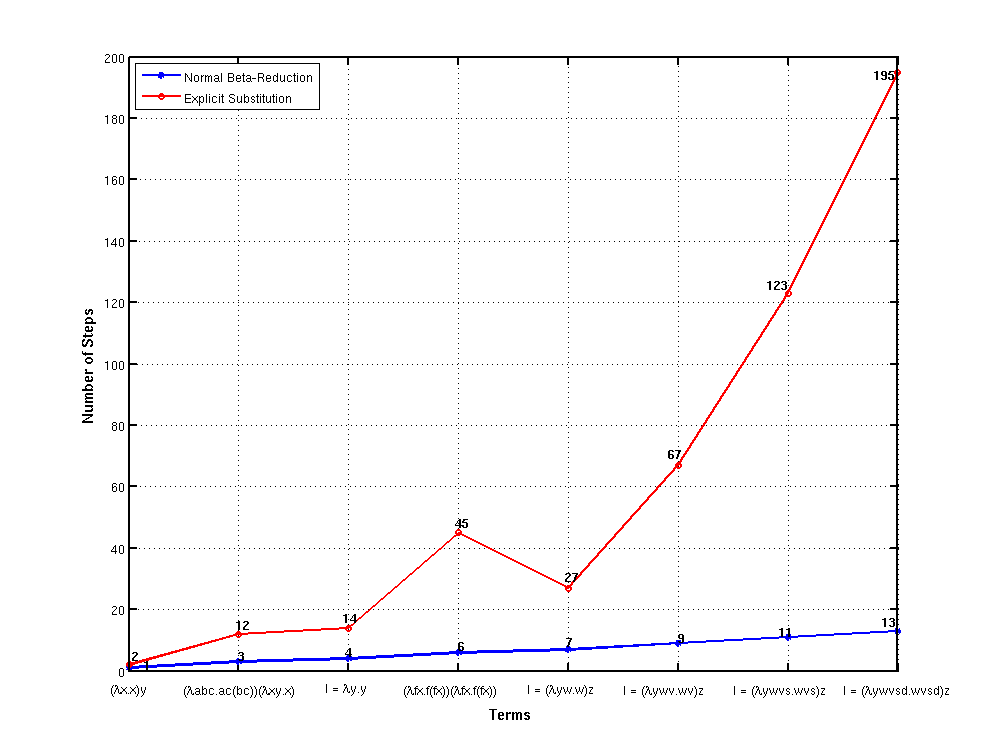
\includegraphics[width=\textwidth]{pics/zhang_01}
\caption{Reduction steps needed for normal $\beta$-reduction and explicit substitution}
\label{fig:betax}
\end{figure}

The figure \ref{fig:betax} illustrates the difference in the number of steps needed between normal $\beta$-reduction and $\xrightarrow[bx]{}$. As the term $I$ grows larger, the number of steps in normal $\beta$-reduction grows linearly, while xgc grows approximately exponentially. We can see that the $\beta$-reduction steps needed for term $(\lambda fx.f(fx))(\lambda fx.f(fx))$ is less than the steps needed when $I = (\lambda yw.w)z$, however, the number of explicit substitution steps is larger. The number of reduction steps mainly depends on the free occurrences of bound variables in an abstraction. For the term $(\lambda fx.f(fx))$, the free occurrence of $f$ and $x$ in $f(fx)$ lead to repeated substitution and increase the number of reduction steps.  


\subsection{$\xrightarrow[\beta ]{}$ vs $\xrightarrow[bx]{}$ vs $\xrightarrow[bxgc]{}$}

The explicit garbage collection simplifies several proofs. For the $\lambda$xgc-term $(xy)\langle z:=M\rangle$, since there is no free occurrence of $z$ in the term $xy$, so the substitution $\langle z:=M\rangle$ can be removed. Then it no longer needs to be pushed into the application $xy$ which costs more explicit substitution steps. The following table and chart would show the number of steps decreased, or in other words, the efficiency improved by garbage collection.  

\begin{table}[h!]
\centering
\begin{tabular}{|c|c|c|c|}\hline
$\lambda$-term & Normal Reduction & Explicit Substitution & bxgc\\ \hline
$(\lambda x.x)y$ & 1 & 2 & 2\\ \hline
$(\lambda abc.ac(bc))(\lambda xy.x)$ & 3 & 12 & 12\\ \hline
$I = \lambda y.y$ & 4 & 14 & 12\\ \hline
$(\lambda fx.f(fx))(\lambda fx.f(fx))$ & 6 & 45 & 45\\ \hline
$I = (\lambda yw.w)z$ & 7 & 27 & 18\\ \hline
$I = (\lambda ywv.wv)z$ & 9 & 67 & 35\\ \hline
$I = (\lambda ywvs.wvs)z$ & 11 & 123 & 58\\ \hline
$I = (\lambda ywvsd.wvsd)z$ & 13 & 195 & 87\\ \hline
\end{tabular}
\caption{Reduction steps needed for normal reduction, explicit substitution, and bxgc}
\label{tb:diffff}
\end{table}

Compared with Table \ref{tb:diff}, Table \ref{tb:diffff} lists additional the number of steps needed by explicit substitution and garbage collection. As we can see, there is no garbage collection performed for the term $(\lambda x.x)y$ and $(\lambda abc.ac(bc))(\lambda xy.x)$. When $I = \lambda y.y$, the garbage collection takes place at the 2nd and 6th reduction step when the term is \verb|\v.((\y.y)<x:=(\y.y)v>)(((\y.y)x)<x:=(\y.y)v>)| and \verb|\v.((\y.y)<x:=(\y.y)v>)(x<x:=(\y.y)v>)|. There is no occurrence of $x$ in \verb|\y.y| in both cases. So the substitution is the garbage and is removed. Therefore, the substitution would no be pushed into the abstraction and it reduces 2 reduction steps.

For the term $(\lambda fx.f(fx))(\lambda fx.f(fx))$, there is no garbage collection performed because of the repeated occurrence of $f$ and $x$. When the term $I$ is gradually enlarged, the number of steps reduced by garbage collection becomes larger. It decreases more than a half when $I = (\lambda ywv.wv)z$. The more the number of reduction steps needed by explicit substitution, the more steps reduced by garbage collection. We can see the difference in Figure \ref{fig:betaxgc}
  
\begin{figure}[h!]
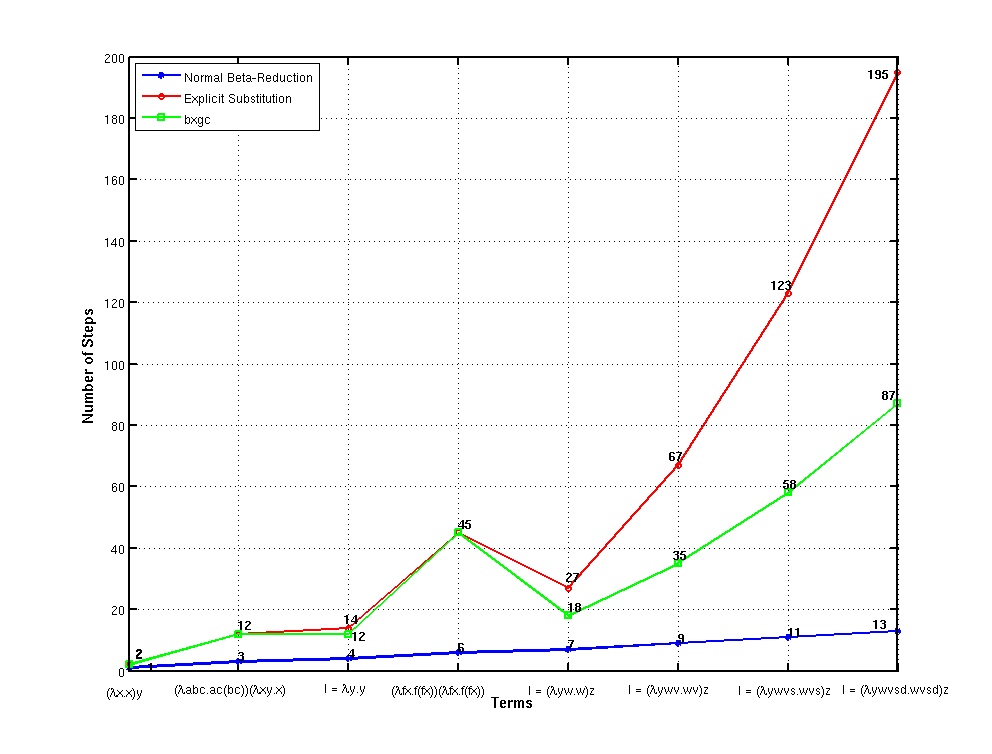
\includegraphics[width=\textwidth]{pics/zhang_02}
\caption{Reduction steps needed for normal reduction, bx, and bxgc}
\label{fig:betaxgc}
\end{figure}


The figure \ref{fig:betaxgc} illustrates the difference in the number of steps needed among normal $\beta$-reduction, $\xrightarrow[bx]{}$, and $\xrightarrow[bxgc]{}$. There is not too much difference between $\xrightarrow[bx]{}$ and $\xrightarrow[bxgc]{}$ for the first 4 terms. The garbage collection has a significant impact as the term $I$ grows larger. As we can see from the graph, the difference between $\xrightarrow[bx]{}$ and $\xrightarrow[bxgc]{}$ becomes larger from $I = (\lambda yw.w)z$ to $I = (\lambda ywvsd.wvsd)z$.

Although the garbage collection can remove any useless substitutions from $\lambda$xgc-terms and avoid redundant explicit substitution steps. It takes much more reduction steps than normal $\beta$-reduction. The number of steps needed by explicit substitution and garbage collection is approximately $nlogn$(only rough estimated).

It is worth mentioning that the reduction path of a term by different reduction strategies also affects the number of reduction steps needed for $\xrightarrow[bx]{}$ and $\xrightarrow[bxgc]{}$. The shortest $\xrightarrow[bxgc]{}$ path of the term $I = \lambda y.y$ is 8, using applicative order reduction. It costs 12 steps for the normal order reduction whereas all the $\beta$-reduction paths of it consist of 4 steps.  




\chapter{The Curry type assignment system}

A type system consists a set of rules that assign a property called a \textit{type} to the various constructs --- such as variable, expression, functions or modules. There are several reasons to add types to a program, one of the most important reason to add type properties to a program is to avoid bugs. It is possible to build an abstract interpretation of programs by treating terms as objects. The abstractions can be regarded as the interface of objects, by checking whether the interfaces have been connected properly we can decide whether the program is defined in a consistent way. Moreover, type systems provide a form of documentation and improve the readability of a program. Since a program can be abstracted, there are less information in the structure of a program. Furthermore, it also enables independent compilation before the implementation of a program runs. The types of functions and arguments can be checked during the generation of codes. Type-checking during implementation enables dynamic  debugging which largely reduces the debugging workload at run-time. If a program is error-free, it is safe to run:``Typed programs cannot go wrong''. It also allows multiple dispatch which is the feature of some objected-oriented programming languages in which a function or method can be dynamically dispatched based on the run time type of more than one of its arguments.
 
An example of a type system is the Java language. A Java program consists of classes which contains a set of function definitions. A function is invoked by an instance of a class that the function belongs to. The interface of a function states the type of the return value, the name of the function and a list of values that are passed to the function. The code of an invoking function states the object instance on which this particular method is to be invoked, and the name of this function along with the names of variables that hold values to pass to it. The Java compiler checks the type of each argument that passed into the function, against the type declared for each varaible in the interface of the invoked function. If the types do not match, the compiler throws a compile-time error.

The lambda calculus as treated in Chapter 1 is referred to as a \textit{type-free} theory. Because every expression may be applied to every other expression. For example, the $\lambda x.x$ may be applied to any argument $x$ and generates the same $x$. 

The typed version of lambda calculus( a variant of the lambda calculus) is introduced essentially in Curry\cite{curry1934functionality}. Types are objects of a syntactic nature and may be assigned to lambda terms. If M is a lambda term and a type A is assigned to M, then we say \textit{`M has type A'}; the notation used is $`M:A'$. For example, in a typed system one has $\lambda x.x : (A \rightarrow A)$, which means the function $\lambda x.x$ should take an argument in type $A$ and return a value of type $A$. In general, $A \rightarrow B$ is the type of functions from $A$ to $B$.

\section{The System $\lambda \rightarrow $-Curry}

In Curry and Feys\cite{curry1972combinatory} and Curry et al\cite{curry1972combinatory2}, the type assignment theory was modified in a natural way to the lambda calculus assigning elements of a given set $\mathbb{T}$ of types to type free lambda terms. For this reason these calculi are sometimes called systems of type assignment. If the type $\sigma \in \mathbb{T}$ is assigned to the term $M \in \Lambda$ which writes as $\vdash M : \sigma$, sometime with a under subcript such as $\vdash _\lambda$ to denote the particular system. Usually a set of assumptions $\Gamma$ is needed to derive a type assignment write as $\Gamma \vdash M : \sigma$(read as `$\Gamma$ yields $M$ in $\sigma$').

\begin{def1}
\normalfont (i) The set of $types$, notation $\mathbb{T}$, 
\end{def1} 

Notation. (i) If $\sigma _1,...,\sigma _n \in \mathbb{T}$ then

\begin{equation*}
\sigma _1 \rightarrow \sigma _2 \rightarrow ... \rightarrow \sigma _n
\end{equation*}

stands for
\begin{equation*}
(\sigma _1 \rightarrow (\sigma _2 \rightarrow ... \rightarrow (\sigma _{n-1} \rightarrow \sigma _n)))
\end{equation*}

we use association to the right, and the rightmost and outermost parentheses are normally omitted. 

(ii) $\alpha,\beta,\gamma,...$ denote arbitrary type variables.



\begin{def1}
\normalfont (i) A \textit{statement} is of the form $M : \sigma$, where $M\in \Lambda$ and $\sigma \in \mathbb{T}$(pronounced as $`M\ has\ type\ \sigma'$). $M$ is called the $subject$ and $\sigma$ the $predicate$ of $M : \sigma$.  
\end{def1}
(ii) A $context$ $\Gamma$ is a set of statements with only distinct (term) variables as subjects; In \cite{svb2001type}, the notion $\Gamma,x:\sigma$ is used for the context $\Gamma \cup \{x:\sigma\}$ where either $x:\sigma \in \Gamma$ or $x$ does not occur in $\Gamma$, and we use $x:\sigma$ as shorthand for $\emptyset,x:\sigma$.

The notion of \textit{context} will be used to collect all statements used for the free variables of a term when typing that term\cite{svb2001type}. 


\begin{def1}\label{def:derivation}
\normalfont (CF. [\cite{curry1934functionality}, \cite{curry1972combinatory}]) \textit{Curry type assignment} and $derivations$ can be defined using following derivation rules.  
\end{def1}
\begin{align*}
&(1):\frac{}{\Gamma ,M:\sigma \vdash _cM:\sigma} \\
&(2):\frac{\Gamma ,x:\sigma \vdash _cM:\beta}{\Gamma \vdash _c(\lambda x.M):\sigma \rightarrow \beta} \\
&(3):\frac{\Gamma \vdash _cM_1:\sigma \rightarrow \beta\ \ \ \ \ \Gamma \vdash _cM_2:\sigma}{\Gamma \vdash _c(M_1M_2):\beta} 
\end{align*}

It is built up from assumptions $x:\sigma$, and it forms a natural deduction system. Following is an example that shows how a statement can be derived by assumptions using deduction rules defined above:

\begin{exmp}\label{exp}
\normalfont (i)Let $\sigma \in \mathbb{T}$. Then $\Gamma \vdash \lambda fx.f(fx):(\sigma \rightarrow \sigma)\rightarrow \sigma \rightarrow \sigma$, is shown by the following derivation:
\end{exmp}

$$
\infer[(2)]{\Gamma \vdash \lambda fx.f(fx):(\sigma \rightarrow \sigma)\rightarrow \sigma \rightarrow \sigma}{
	\infer[(1)]{\Gamma \vdash \lambda x.f(fx):\sigma \rightarrow \sigma}{
      \infer{\Gamma \vdash f(fx):\sigma}{
             \infer[(1)]{\Gamma,f:\sigma \rightarrow \sigma \vdash f:\sigma \rightarrow \sigma}{}
             & 
             \infer{\Gamma \vdash fx:\sigma}{
                \infer{\Gamma,f:\sigma \rightarrow \sigma \vdash f:\sigma \rightarrow \sigma}{}
                &
                \infer{\Gamma,x:\sigma \vdash x:\sigma}{}
             }
         }
      }		
	}
$$


(ii)Notice that, we cannot type \textit{`self-application'} $xx$. In order to type the application $xx$, the derivation should be as following:

$$
\infer{\Gamma \vdash xx:B}{
    \infer{\Gamma \vdash x:A \rightarrow B}{} 
    &
    \infer{\Gamma \vdash x:A}{}
}
$$


As we can see, the term variable $x$ is assigned to two types: $A \rightarrow B$ and $A$, and neither of them can be substituted by the other one. So, $A \rightarrow B \neq A$, and there are two statements of subject $x$ in context $\Gamma$ with distinct predicates. Those two statements would be conflict according to the definition of context. Therefore, the `self-application' is untypable. 


\section{Properties of $\lambda \rightarrow $}

\begin{lemma}
\normalfont (Barendregt \cite{barendregt1984introduction}) GENERATION LEMMA
\end{lemma}
\begin{align*}
  &(i)\ \Gamma \vdash x:\sigma \Rightarrow (x:\sigma)\in \Gamma \\
  &(ii)\ \Gamma \vdash MN:\gamma \Rightarrow \exists \sigma[\Gamma \vdash M:(\sigma \rightarrow \gamma)\ \& \ \Gamma \vdash N:\sigma]\\
  &(iii)\ \Gamma \vdash \lambda x.M:\rho \Rightarrow \exists \sigma ,\gamma[\Gamma ,x:\sigma \vdash M:\gamma\ \& \ \rho \equiv (\sigma \rightarrow \gamma)] 
\end{align*}


\begin{lemma}
\normalfont (van Bakel \cite{svb2001type}) SUBSTITUTION LEMMA
\end{lemma}
\begin{align*}
   \exists \sigma[\Gamma,x:\sigma \vdash M:\gamma \ \& \ \Gamma \vdash N:\sigma]\Rightarrow M[x:=N]:\gamma
\end{align*}

Proof by induction on the derivation of $\Gamma,x:\sigma \vdash M:\gamma$.

\begin{theorem}
\normalfont (Barendregt \cite{barendregt1984introduction}) \textsc{SUBJECT REDUCTION THEOREM}
\end{theorem}

\textit{Suppose M $\twoheadrightarrow$ M'. Then} 
\begin{align*}
   \Gamma \vdash M:\sigma \Rightarrow \Gamma \vdash M':\sigma
\end{align*}

\noindent PROOF (Barendregt \cite{barendregt1984introduction}).

\begin{align*}
   &\Gamma \vdash (\lambda x.M)N:\sigma & \Rightarrow \mathrm{(Generation lemma)}\\
   &\Gamma \vdash (\lambda x.M):\gamma \rightarrow \sigma \& \Gamma \vdash N:\gamma &  \Rightarrow \mathrm{(Generation Lemma)}\\
   &\Gamma ,x:\gamma \vdash M:\sigma \& \Gamma \vdash N:\gamma & \Rightarrow \mathrm{ (Substitution Lemma)}\\
   &\Gamma \vdash M[x:=N]:\sigma
\end{align*} 



\section{The principal type property}

The principal type schemes for Curry's system were first defined in \cite{hindley1969principal}. The principal type property indicates that, amongst all the types that can be assigned to a term, there is a `principal' one that all other types can be created from it. The types are `created' by substitution rules which defines the operation that a type variable is replaced by a type in a consistent way.


\begin{def1}{\label{def:tsub}}
\normalfont (Type substitution(van Bakel\cite{svb2001type})) a) The substitution $(\varphi \mapsto C): $, where $\varphi$ is a type variable and $C \in \mathbb{T}$ is defined as following:
\end{def1}

\begin{equation*}
\begin{array}{ll}
(\varphi \mapsto C)\varphi        & = C\\
(\varphi \mapsto C)\varphi '      & = \varphi ',if\ \varphi '\neq \varphi\\
(\varphi \mapsto C)A\rightarrow B & = ((\varphi \mapsto C)A)\rightarrow ((\varphi \mapsto C)B)
\end{array}
\end{equation*}

b) If $S_1$, $S_2$ are substitutions, then So is $S_1\circ S_2$, where $S_1\circ S_2A=S_1(S_2A)$

c) \texttt{S}$\Gamma = \{x:$\texttt{S}$B | x:B \in \Gamma\}$

d) $S\langle \Gamma, A\rangle=\langle S\Gamma, SA\rangle$

For the Curry type assignment system, the principal type property is expressed by: for each typeable term $M$, there exists a \textit{principal pair} of context $\Pi$ and type $P$ such that $\Pi \vdash M:P$, and for all context $\Gamma$, and types $A$, if $\Gamma \vdash M:A$, then there exists a substitution \texttt{S} such that \texttt{S}$\Pi=\Gamma$ and \texttt{S}$P=A$ \cite{svb2001type}.

In type theory, \textit{Polymorphism} is an important feature of programming languages. Polymorphism enables different types of entities implements the same interface but with different properties. A polymorphic type is a type whose operations can also be applied to values of some other type, or types. The principal type property for type assignment system plays an important role in programming languages that model polymorphic functions.   

Principal types for $\lambda$-terms are defined using the notion of unification of types that was defined by Robinson in \cite{robinson1965machine}. Given two types, the unification operation always maps the arguments to a smallest common instance with respect to substitution. It can be defined as follows:

\begin{def1}\label{eq:rob}
\normalfont (van Bakel \cite{svb2001type}) Let $Id_s$ be the substitution that replaces all type variables by themselves:
\end{def1}

\noindent (i) Robinson's unification algorithm. Unification of Curry types is defined by:

\begin{equation*}
\begin{array}{llll}
\mathrm{unify} & \varphi            & \varphi          & = (\varphi \mapsto \varphi)\\
\mathrm{unify} & \varphi            & B                & = (\varphi \mapsto B), if\ \varphi \mathrm{\ does\ not\ occur}\ in\ B\\
\mathrm{unify} & A                  & \varphi          & = \mathrm{unify}\ \ \varphi\ \ A\\
\mathrm{unify} & (A\rightarrow B)   & (C\rightarrow D) & = S_1\circ S_2\\
&&&\ \ \ \mathrm{unify}\ S_1 = \mathrm{unify}\ \ A\ \ C\\
&&&\ \ \ \ \ \ \ \ \ \ \ S_2 = \mathrm{unify}\ (S_1B)\ (S_1D)
\end{array}
\end{equation*}


\noindent (ii) By defining the operation \texttt{UnifyContexts}, the operation \texttt{unify} can be generalised to contexts:

\begin{equation*}
\begin{array}{llll}
\mathrm{UnifyContexts} & (\Gamma _0,x:A) & (\Gamma _1,x:B) & = S_1\circ S_2\\
&&&\ \ \ \mathrm{where}\ S_1 = \mathrm{unify}\ \ A\ \ B\\
&&&\ \ \ \ \ \ \ \ \ \ \ \ S_2 = \mathrm{UnifyContexts}\ (S_1\Gamma _0)\ (S_1\Gamma _1)\\
\mathrm{UnifyContexts} & (\Gamma _0,x:A) & \Gamma _1 & = \mathrm{UnifyContexts}\ \Gamma _0\ \Gamma _1, \mathrm{if\ x\ does\ not\ occur\ in\ \Gamma _1}\\
\mathrm{UnifyContexts} & \varnothing & \Gamma _1 & =  Id_s
\end{array}
\end{equation*}


In order to find the principal pair for $\lambda$-terms, the principal pair algorithm is introduced. The principal algorithm defined below in Definition \ref{def:ppc}


\begin{def1}{\label{def:ppc}}
\normalfont (van Bakel \cite{svb2001type}) Principle  Pair  Algorithm  for  $\Lambda$
\end{def1}

\begin{equation*}
\begin{array}{llll}
pp_c & x & = & \langle x:\varphi,\varphi \rangle\\
&&& \mathrm{where}\ \ \varphi=\mathrm{fresh}\\
pp_c & (\lambda x.M) & = & \langle \Pi,A \rightarrow P \rangle,\ \mathrm{if}\ pp_c\ M=\langle \Pi \cup \{x:A\},P \rangle\\
&&& \langle \Pi,\varphi \rightarrow P \rangle,\ \mathrm{if}\ pp_c\ M=\langle \Pi ,P \rangle\ \ \ \ x\not\in \Pi\\
&&&\ \ \ \ \ \ \ \ \ \ \ \ \ \ \ \ \ \mathrm{where}\ \varphi=\mathrm{fresh}\\
pp_c & (MN) & = & S_1\circ S_2\langle \Pi _1\cup \Pi _2,\varphi \rangle\\
&&& \mathrm{where}\ \ \ \varphi \ \ \ \ \ \ \ = \mathrm{fresh}\\
&&& \ \ \ \ \ \ \ \ \ \ \langle \Pi _1,P_1\rangle = pp_c\ M\\
&&& \ \ \ \ \ \ \ \ \ \ \langle \Pi _2,P_2\rangle = pp_c\ N\\
&&& \ \ \ \ \ \ \ \ \ \ S_1 \ \ \ \ \ \ \ = \mathrm{unify}\ P_1\ \ (P_2 \rightarrow \varphi)\\
&&& \ \ \ \ \ \ \ \ \ \ S_2 \ \ \ \ \ \ \ = \mathrm{UnifyContexts}\ (S_1\Pi _1)\ (S_1\Pi _2)\\
\end{array}
\end{equation*}

\section{Typing $\lambda$xgc-terms}

Since we have extended the lambda calculus by the explicit substitution and garbage collection, $\lambda$xgc-terms also need to be typed. On the basis of the ordinary Curry type assignment system, we add a new derivation rule and the principal pair algorithm for $\lambda$xgc-term in the form  $M\langle x:=N\rangle$.

\begin{def1}
\normalfont \textit{($\lambda$xgc-term type assignment)} $derivations$ can be defined using following derivation rule.  
\end{def1}
\begin{equation*}
(4):\frac{\Gamma, {x:\sigma} \vdash M:\beta\ \ \ \ \ \Gamma \vdash _cN:\sigma}{\Gamma \vdash _cM\langle x:=N\rangle \beta} 
\end{equation*}

Notice that, here we only list the derivation rule that has been added to the ordinary derivation rules defined in Definition \ref{def:derivation}. Therefore, the derivation rules 1,2,3,4 forms the derivation rule set for $\lambda$xgc-calculus.

In $M\langle x:=N\rangle$, $x$ can be substituted by $N$, so they must have the same type. Then substitute all the free occurrence of $x$ in $M$ will not change the type of $M$. 


\begin{def1}{\label{def:ppcxgc}}
\normalfont  Principle  Pair  Algorithm  for  $\Lambda$x
\end{def1}


\begin{equation*}
\begin{array}{llll}
pp_c & (M\langle x:=N\rangle) & = & S_1\circ S_2\langle \Pi _1\cup \Pi _2,P_1 \rangle \ \ \ \mathrm{if}\ x\ \not\in FV(M)\\
&&& S_1\circ S_2\langle \Pi _3\cup \Pi _2,P_1 \rangle \ \ \ \mathrm{if}\ x\ \in FV(M)\\
&&& \mathrm{where} \ \ P_3 \ \ \ \ \ \ \ = \mathrm{fresh} \ \ \ \ \ \ \ \ \ \ \ \ \ \mathrm{if}\ x\ \not\in FV(M)\\
&&& \ \ \ \ \ \ \ \ \ \ \Pi _1 \ \ \ \ \ \ \ = \Pi _3 \cup \{x:P_3\}\ \ \ \mathrm{if}\ x\ \in FV(M)\\
&&& \ \ \ \ \ \ \ \ \ \ \langle \Pi _1,P_1\rangle = pp_c\ M\\
&&& \ \ \ \ \ \ \ \ \ \ \langle \Pi _2,P_2\rangle = pp_c\ N\\
&&& \ \ \ \ \ \ \ \ \ \ S_1 \ \ \ \ \ \ \ \ = \mathrm{unify}\ P_2\ \ P_3\\
&&& \ \ \ \ \ \ \ \ \ \ S_2 \ \ \ \ \ \ \ \ = \mathrm{UnifyContexts}\ (S_1\Pi _1)\ (S_1\Pi _2)\\
\end{array}
\end{equation*}


Based on the ordinary principal pair algorithm, we add the algorithm for $\lambda$xgc-term in the form $M\langle x:=N\rangle$. The type of term $M\langle x:=N\rangle$ is eventually the type assigned to $M$. Recall that, the context is used to collect all the statements used for the free variables of a term when typing that term. If $x$ is a free variable in $M$, the statement of $x$ in $\Pi_1$ should be removed.




















  


\chapter{A Purely-Functional Programming Language --- Haskell}

This chapter will introduce functional programming and a purely-functional programming language-Haskell. It will demonstrate how the lambda calculus and Curry type assignment system is implemented in Haskell by self-defined data types, pattern matching, list processing, and recursive functions. As an implementation and usable software, the issues and weaknesses would also be discussed in this chapter. 
\section{Functional Programming}
Functional programming uses functions, other than objects or procedures, as the fundamental building blocks of a program. It is a programming paradigm that treats computation as the evaluation of expressions and avoids mutable data and state, in contrast with imperative programming where programs are composed of statements which change global state when executed. Functional programming has its roots in lambda calculus. Lambda calculus provides a theoretical framework for describing functions and their evaluation. Although it is a mathematical abstraction rather than a programming language, it forms the basis of almost all functional programming languages. There are several functional programming languages such as Miranda, Haskell, and OCaml that is defined based on lambda calculus. 
\section{Haskell}
Haskell is an advanced purely-functional programming language, which has non-strict semantcis and strong static typing. In imperative languages(C, C++, Java...), a sequence of tasks are generated and executed in a program. When they are executed, it can change state. It has a control flow structures for doing some action several times. In purely functional programming, we do not need to tell the computer what to do but rather to tell it what each function is. It also cannot set a variables to something and then set it to something else later. In purely functional languages, a function has no side-effects. The only task for a function is to take the arguments, perform operations, and return the result.  

Haskell is lazy, which means that it will not execute functions and calculate things unless it is specifically told to do so. If you compile and run a haskell program, it does not call any functions nor perform any execution. The only thing you can do is call a specific function(it may call other functions) and pass parameters into it, then that function is executed and a result is returned.   

Haskell is statically typed. When we compile a haskell program, the compiler knows which variable is a number, which is a string and so on. That means errors can be found at compile time. Haskell uses a type system that has type inference. That means we do not have to explicitly label every piece of code with a type because the type system can automatically type it. Type inference also allows the code to be more general. If we add two parameters together without explicitly stating their types, the function will work on any two parameters that can be added as numbers. 

Haskell is elegant and concise, because it uses a lot of high level concepts. Haskell programs are usually shorter than their imperative language equivalents. In addition, shorter programs are easier to develop than longer ones and have less bugs. 

In this project, Haskell is self-studied thanks to the course note of COMP120.1 of Imperial College. In this section, some main features of Haskell would be introduced by examples.

\subsection{Pattern Matching}
Pattern matching consists of listing patterns to which some data should conform and then checking to see if it does conform to any of them and deconstructing the data according to those patterns. When defining functions, we can define separate function bodies for different patterns. This leads to really neat code that is simple and readable. We can pattern match on any data type. A successful match binds the formal parameters in the pattern. The matching process itself occurs ``top-down'' and ``left-right''. Failure of a pattern anywhere in one function body results in failure of the whole matching process, and the next function body is then tried to match. For instance, if [2, 3] is matched against [1, a], then 2 fails to match with 1, so the result is a failed match. Following is another example that defines a function using pattern matching:

\begin{verbatim}
                     factorial :: (Integral a) => a -> a  
                     factorial 1 = 1
                     factorial n = n * factorial (n-1)
\end{verbatim}

The code above defines a funtion that calculate the factorial of the input. It uses pattern matching that lists all the possible patterns that can be matched. Here, only two cases, 1 or n. It firstly matches the first function body to check whether the input is 1; if not, goes to next function body and calls itself again.   

\subsection{Guards}

Patterns are used to specify data should form to some form and deconstruct it, whereas guards are used to check whether some properties of an argument are true or false. It is similar to an if statement, and more likely to a `swtich' block in Java. Following is an example of using guards:
\begin{verbatim}
                     max :: (Ord a) => a -> a -> a
                     max a b | a > b     = a
                             | otherwise = b
\end{verbatim}
The function above returns the maximum value between the inputs $a$ and $b$. Notice that, `Ord' here enables ordering on a general type a, so we can apply `>' `<' to compare two variables in type a.

\subsection{Where}

The `where' block is used to simplify complex codes with newly defined variables. It avoids repeated expressions: an expression is only calculated onece and it is binded to a name than then the name can be referred to instead of the whole expression. 

\begin{verbatim}
                    divA :: Float -> Char
                    divA a | a/2 <= 10  = 'A' 
                           | a/2 <= 20  = 'B'
                           | a/2 <= 30  = 'C'
                           | otherwise  = 'D'
\end{verbatim}

The function above firstly calculte the input parameter $a$ divided by 2, and decides which sector it is in and returns a character. It repeatly defines the expression \verb|a/2| for three times. We can avoid that by using `where' statement as below: 
\begin{verbatim}
                    divA :: Float -> Char
                    divA a | b > 10  = 'A' 
                           | b > 20  = 'B'
                           | b > 30  = 'C'
                           | otherwise = 'D'
                           where b = a/2
\end{verbatim}

As we can see, it improves the readability by giving names to an expression and can accelerate programs since expressions like \verb|a/2| is calculated only once. Mention that, these names like \verb|b| are visible across the guards. 

\subsection{Self-defined Types}

We can also create our own data types in a very straight forward way. One way is to use the \textbf{data} keyword.

\begin{verbatim}
        data Bool = False | True
\end{verbatim} 

\verb|data| means that we are defining a new data type. The part one the left of \verb|=| denotes the type name, which is \verb|Bool|. The parts after the \verb|=| are value constructors. They specify the different values that this type can have. 



\section{Model the $\lambda$-calculus and the Curry Type Assignment System in Haskell}
\section{Issues and Weakness of Implementation in Haskell }


\chapter{The $\lambda$-calculus and Curry Type Assignment System Implementation in Java}
The Java version of implementation is transferred directly from Haskell. However, the semantics and operational order of Haskell is difference from Java, especially the `where' statement of Haskell. The 'where' declaration is called when the defined variables are used, however, in Java, we need to separate a `where' block into parts according to where it is called. An example is shown in Section \ref{sec:hj}. This differece is worth taking care of when transfer the Haskell into Java, otherwise, NullPointerException may occur. 

In all data types, the method toString() has been implemented -- more precisely overridden, as it is a method of the Java primary class\verb| Object|. This function is used to print out the data type as a string. There are more method signatures defined in the interfaces as a reference to instantiable classes. 

\section{Different operational order between Haskell and Java}{\label{sec:hj}}
As mentioned above, the operaional order of Haskell is different from Java, not only the pattern matching, but also the `where' declarations. Since the code in Haskell cannot be transferred into Java directly, it largely abandoned the simplicity of codes. Following is a piece of code that defines principle pair algorithm:
\begin{verbatim}
ppc :: Term -> [Char] -> (PPc, [Char])
ppc (Abs x y) r | contains (Var x) pi = ((removeItem (Var x, a) pi, (TP a p)), tl1)
                | otherwise = ((pi, (TP f p)), tl1)
                            where (f, tl) = fresh r                    (1) 
                                  ((pi, p), tl1) = ppc y tl            (2)
                                  (_, a) = search (Var x) pi           (3)

\end{verbatim}

`Guards' are used as an if-then-else block. There are three declarations in the `where' block each with a distinct number. For the first condition of ppc function, declaration (1)(2)(3) are called since all the declared variables are used. In the `otherwise' condition, only declaration (1)(2) are called. In this case, in order to transfer the Haskell function into Java methods, we need to repetitively define the variables which largely reduces the simplicity of codes. 





\begin{verbatim}
public PPC ppc(Term term, String counter){
     ...
     else if(term instanceof Abstraction){
        Variable xv = new Variable(((Abstraction) term).getName());
        PPC receiver = ppc(((Abstraction) term).getTerm(), counter);
        if(receiver != null){
           if(contains(xv, receiver.getSubject())){
             Type searchType = search(xv, receiver.getSubject()).getPredicate();
             ArrayList<Statement> original = receiver.getSubject().getContext();
             ArrayList<Statement> remove = new ArrayList<>();

             for(Statement s: original){
               if(s.getSubject().equals(xv)) remove.add(s);
             }

             for(Statement rm: remove){
                original.remove(rm);
             }

             TP tp = new TP(searchType, receiver.getPredicate());
             return new PPC(new Context(original), tp, receiver.getCounter());
          }
          else{
             TVar f = new TVar(receiver.getCounter().substring(0, 1));
             return new PPC(receiver.getSubject(), new TP(f, receiver.getPredicate()),
                            receiver.getCounter().substring(1));

          }
       }
       else {
           return null;
       }
     }
     ...
}
\end{verbatim}

\section{$\lambda$-calculus Representation}
\subsection{$\lambda$-terms}
A Lambda term can either be a variable, an abstraction or an application. An interface `Term' is defined as a reference type, which has three lambda term implementations. This is the generic representation of all lambda terms.

\begin{figure}[ht]
\centering
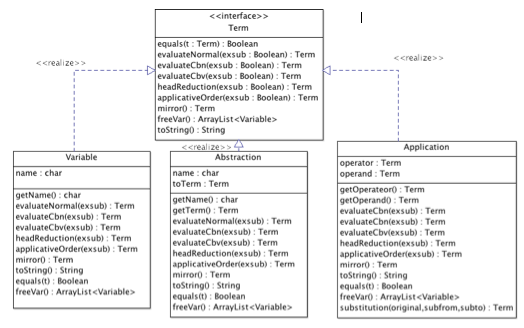
\includegraphics[scale=0.7]{pics/Term}
\caption{Class diagram of Lambda Calculus data structures}
\label{fig:term1}
\end{figure}

This interface defines the method \verb|equals(Term t)|, which return a boolean states whether it is equal to the input term. This method overrides the \verb|equals(Object o)| method of the Java primary class \verb|Object|. It is essential in the reduction procedure, since we can decide whether a term is reducible by compare the term before reduction and after. If the term is the same as it before reduction, then it cannot be reduced. Therefore, we know when we can stop the reduction procedure.  

As mentioned in Section \ref{sec:reductionstrategy}, there are five reduction strategies enabled in the reducer. So there are five method signatures defined in the interface: \textsf{evaluateNormal(Bool exsub), evaluateCbn(Bool exsub), evaluateCbv(Bool exsub), headReduction(Bool exsub), applicativeOrder(Bool exsub)}. Each of these method refers to a specific reduction strategy as the method name. 

The method \textsf{mirror()} is used to create a mirror term with exactly the same class variables. This method is used when the substitution is performed. For example, if we have a lambda term $\lambda f.(\lambda x.f(xx))(\lambda x.f(xx))$, it is reduced to $\lambda f.f((\lambda x.f(xx))(\lambda x.f(xx)))$. If we do not create a mirror term of $(\lambda x.f(xx))$, both of these two $(\lambda x.f(xx))$ would refer to the same memory space. In other words, the abstraction $(\lambda x.f(xx))$ is used twice to form an application. Therefore, if operations performed on the function, it is also performed on the argument. It is essential to create a mirror term that separate those two terms although they look exactly the same.

The method \textsf{freeVar()} is used to get all the free variables of a $\lambda$-term. It is used to perform $\alpha$-conversion when we substitute bound variables in an abstraction. The free variables are defined in Definition \ref{eq:fv}.       

Finally, the \textsf{toString()} method of class \textsf{Object} is overridden to transform a lambda term to a string. 

Notice that, in the implementation class \verb|Application|, there is a \textsf{substitution(Term original, Term subfrom, Term subto):Term} method. It is used to substitute bound variables in an abstraction, which is an application function, to the argument. The first parameter of the method is the body of abstraction, the second argument states which bound variable could be substituted and the third argument states what it could be substituted to.

\subsection{Interpreter}
To allow interactions and inputs from users, the program needs to interpret the input term into a data structure in the system. Figure \ref{fig:inter} illustrates all the methods that used to interpret an input into a lambda term data structure.   

\begin{figure}[ht]
\centering
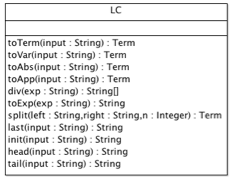
\includegraphics[scale=0.6]{pics/LC}
\caption{Interpretation methods in LC class}
\label{fig:inter}
\end{figure}

The method \textsf{toTerm(String input)} takes a string as input and returns a \textsf{Term}. It calls \textsf{toVar(String input), toAbs(String input)} or \textsf{toApp(String input)} according to type of the outermost term. Then, those three methods iteratively call each other until the whole term is interpreted.   

\textsf{div(String exp)} divides an application into the function and argument. Basically, it return an array with 2 string elements. The method \textsf{toExp(String exp)} is used to remove brackets of applications and returns an expression that is bracker-free. Finally, the most important method \textsf{split(String left, String right, Int n)} implements the bracket removal mechanism. It marks the right most right bracker `)' and find the matching left bracket `(' and extract the term out without brackets.

Since the Java implementation is directly transferred from Haskell, there are also four basic string operations which are Haskell builit-in functions. \textsf{last(String input)} takes a string and returns the last character of the string, it returns itself if the length of input string is 1. \textsf{init(String input)} accepts a string and returns the string without its last character, it returns an empty string if it only contains one character. \textsf{head(String input)} takes a string and returns the first element of the string, it returns itself when the input string length is 1. \textsf{tail(String input)} takes a string and returns the string without its first element, it returns an empty string when the length of input is 1. 

Following is the example of how those Haskell built-in function work:

\begin{verbatim}
              init "Hello"   "Hell"            head "Haskell"   "H" 
              init "A"       ""                head "A"         "A"
\end{verbatim}

\begin{verbatim}
              last "String"   "g"              tail "Lambda"   "ambda" 
              last "A"        "A"              tail "A"         ""
\end{verbatim}


\section{Curry Type Assignment System Representation}


\subsection{Types}{\label{subsec:types}}

\begin{figure}[ht]
\centering
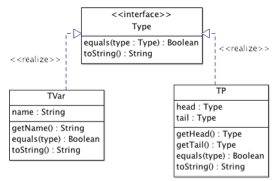
\includegraphics[scale=0.7]{pics/Type}
\caption{Class diagram of type representation}
\label{fig:type}
\end{figure}

Type assignment system assigns types to $\lambda$-terms. In $\mathbb{T}$, a type can either be a single type($A,B,...$) or a complex type($A\rightarrow B$). Since the complex type is formed by single types, it can be represented using the binary tree structure, where single types are leafs and complex types are branches. For example, the type $(A\rightarrow B)\rightarrow C$ is represented as \textsf{TP(TP (TVar A)(TVar B))(TVar C)}, or in a more intuitionistic way:

\Tree 
[.TP [.TP A B ] C ]

Illustrated in Figure \ref{fig:type}, the interface \textsf{Type} is defined as a reference type. It defines two basic method signatures: \textsf{equals(Type type)} and \textsf{toString()} which override the primary methods in \textsf{Object}. There are two implementation class: \textsf{TVar} and \textsf{TP} which stand for single type and complex type. \textsf{TVar} contains a class variable \textsf{name} which states the type name. It implements method signatures defined in the interface and a get method that returns the type name. The implementation class \textsf{TP} is similar to a \textsf{Node} of a tree structure, which contains two class variables: left branch and right branch. Method signatures and get methods are implemented in the class.

\subsection{Type substitution}

Principal types for $\lambda$-terms are defined using the notion of unification of types that defined by Definition \ref{eq:rob}. Similar to types structure in Section \ref{subsec:types}, a type substitution can either be a single substitution($\varphi  \mapsto B$) or a complex substitution($S_1 \circ S_2$). It could also be represented as a binary tree structure. For example, when we unify $(A\rightarrow B)\rightarrow C$ and $(A\rightarrow D)\rightarrow E$, we would get the complex substitution$((A \mapsto A)\circ (B \mapsto D))\circ (C \mapsto E)$ which also can be represented as a binary tree:

\Tree 
[.So [.So $(A\mapsto A)$ $(B\mapsto D)$ ] $(C\mapsto E)$ ]

As shown in Figure \ref{fig:tsub}, an interface \textsf{TSub} is needed as a reference type. It doesnt have any method signatures, operation on substitutions are defined as auxiliary function in class \textsf{LC}.

\begin{figure}[ht]
\centering
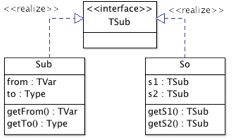
\includegraphics[scale=0.7]{pics/TSub}
\caption{Class diagram of type substitutions representation}
\label{fig:tsub}
\end{figure}
\subsection{Other data types}

The Curry type assignment system defines other concepts besides types and substitutions. Statement is essential to describe the type assigned to a $\lambda$-term; Context is used to collect all statements used for free variables of a term when typing that term; and PPC is a data type that stores context and the type assigned to that term typed. 

\begin{figure}[ht]
\centering
\begin{minipage}{.3\textwidth}
\centering
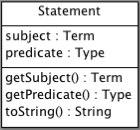
\includegraphics[scale=0.6]{pics/Statement}
\caption{Class diagram of Statement}
\label{fig:statement}
\end{minipage}\hfill
\begin{minipage}{.3\textwidth}
\centering
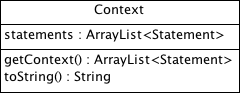
\includegraphics[scale=0.6]{pics/Context}
\caption{Class diagram of Context}
\label{fig:context}
\end{minipage}\hfill
\begin{minipage}{.3\textwidth}
\centering
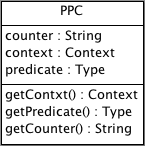
\includegraphics[scale=0.5]{pics/PPC}
\caption{Class diagram of PPC}
\label{fig:ppc}
\end{minipage}
\end{figure}

The \textsf{Statement} class has two attributes which are subject and predicate. It contains basic get method that return \textsf{private} attributes, and it also overrides the \textsf{toString()} method to transform a \textsf{Statement} into a string as ``subject : predicate''

The \textsf{Context} class only contains an \textsf{ArrayList} of \textsf{Statement} as attribute. A context could have none statement if all the variables are bound. The \textsf{toString()} method returns the context a string in the format: ``statement1, statement2, ...'' 

The \textsf{PPC} class, storing principle pair algorithm results, is a little more complex. As defined in Definition \ref{def:ppc}, the ppc function return a context and the type assigned to the term typed as $\langle$context, type$\rangle$. A PPC instance, stores the result of ppc function, therefore it contains two attributes as context and type. In additional, it also has a counter attribute. Since principle pair algorithm always create \textsf{fresh} types, we should keep track of what type names are available that have not been used. It basically states all the available type names.   

\subsection{Core type assignment mechanism implementation}

The Curry type assignment implementation is built based on the lambda calculus implementation. As it extends more operation on $\lambda$-terms for type assignment, there are more auxiliary methods defined in class \textsf{LC}. 

\begin{figure}[ht]
\centering
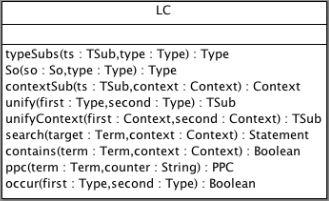
\includegraphics[scale=0.6]{pics/LCType}
\caption{Class diagram of Lambda Calculus data structures}
\label{fig:lctype}
\end{figure}


The methods listed in Figure \ref{fig:lctype} are the core type assignment mechanism implementations. The top-level method is \textsf{ppc(Term term, String counter)}, when a term comes in and needs to be typed, the ppc method is called and it iteratively calls other auxiliary methods. Finally, it will return a \textsf{PPC} instance which contains a context and the typed assigned. 

Given a type substitution and a type, the method \textsf{typeSubs(TSub, Type)} substitutes all the type variables according to the subsitution. It implements the type substitution defined in Definition \ref{def:tsub}. Notice that, since a \textsf{TSub} can either be a single substitution \textsf{Sub} or a complex \textsf{So} as defined in Section \ref{fig:tsub}, it calls \textsf{So(So, Type)} method that implements the \textsf{So} substitution described in Definition \ref{def:tsub} (b). 

The method \textsf{contextSub(TSub, Context)} implements the context substitution defined in Definition \ref{eq:rob} (c). 

The method \textsf{unify(Type, Type)} implements the type unification algorithm defined in Definition \ref{def:tsub}. And \textsf{unifyContext(Context, Context)} implements the context unification in Definition \ref{eq:rob} (ii). It should be mentioned that, since $Id_s$ stands for the substitution that replaces all type variables by themselves, it could be simplified as a substitution that only contains the substitution $(A\mapsto A)$. We do not care what the type $A$ is and whether it is a valid type variable, becuase the substitution $(A\mapsto A)$ would not affect any unifications. 

The \textsf{search(Term, Context)} methods is an auxiliary method that given a $\lambda$-term and a context, it returns the corresponding statement of that term in the context. This method is used in two places. Firstly, it is used when we want to unify the context $\Gamma_0$ and $\Gamma_1$. We need to find the statements with the same subject in these two context and unify them. Therefore, when we traverse through the context $\Gamma_0$, the search method is neccessary to find the corresponding statement in $\Gamma_1$. Secondly, it is used in the principal pair algorithm when we type an abstraction. The temporary type assigned to bound variables should be removed from the context. Therefore, given a variable, the search method can find the corresponding statement and further be removed.  

The method \textsf{contains(Term, Context)} takes a $\lambda$-term and a context as arguments and return a boolean states whether the context contains a statement for the term.

\textsf{ppc(Term, String)} is the core principal pair algorithm implementation method. The definition of principal pair algorithm can be found in Definition \ref{def:ppc}. The second argument in \textsf{String} type is the counter of all available type names. 

Finally, the method \textsf{occur(Type, Type)} is used to decide whether a type occurs in another. It is used in the second type unificatin algorithm defined in Definition \ref{eq:rob}.

\section{Explicit substitution and garbage collection}

\begin{figure}[ht]
\centering
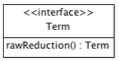
\includegraphics[scale=0.7]{pics/TermRaw}
\caption{Class diagram of Lambda Calculus data structures}
\label{fig:termraw}
\end{figure}
\section{Syntax}
\chapter{GUI development}

\section{Layout}

\section{Functionalities}
\chapter{Haskell vs Java, Pros and Cons}

Having implemented the lambda calculus, reduction strategies, $\lambda$xgc-calculus, and Curry type assignment system in both Haskell and Java, one question would arise: what is the advantage of using Haskell instead of Java. This chapter would compare the features of Haskell and Java and expose the pros and cons of using Haskell upon Java. 

\section{Pros}
\subsection{Concise and elegant}



\section{Cons}
\chapter{Conclusion}



\bibliographystyle{plain}
\bibliography{ref}

\end{document}